% Copyright (c) 2014 by the University of Waikato, Hamilton, NZ. 
% This work is made available under the terms of the 
% Creative Commons Attribution-ShareAlike 4.0 license,
% http://creativecommons.org/licenses/by-sa/4.0/.
%
% Version: $Revision$

\documentclass[a4paper]{book}

\usepackage{wrapfig}
\usepackage{graphicx}
\usepackage{hyperref}
\usepackage{multirow}
\usepackage{scalefnt}
\usepackage{tikz}

% watermark -- for draft stage
\usepackage[firstpage]{draftwatermark}
\SetWatermarkLightness{0.9}
\SetWatermarkScale{5}

% Copyright (c) 2009 by the University of Waikato, Hamilton, NZ. 
% This work is made available under the terms of the 
% Creative Commons Attribution-ShareAlike 3.0 license, 
% http://creativecommons.org/licenses/by-sa/3.0/. 
%
% Version: $Revision: 2916 $

\newenvironment{tight_itemize}{
\begin{itemize}
  \setlength{\itemsep}{1pt}
  \setlength{\parskip}{0pt}
  \setlength{\parsep}{0pt}}{\end{itemize}
}

\newenvironment{tight_enumerate}{
\begin{enumerate}
  \setlength{\itemsep}{1pt}
  \setlength{\parskip}{0pt}
  \setlength{\parsep}{0pt}}{\end{enumerate}
}

% if you just need a simple heading
% Usage:
%   \heading{the text of the heading}
\newcommand{\heading}[1]{
  \vspace{0.3cm} \noindent \textbf{#1} \newline
}

\newcommand{\icon}[1]{\tikz[baseline=-3pt]\node[inner sep=0pt,outer sep=0pt]{\includegraphics[height=1.1em]{#1}};}


\title{
  \textbf{ADAMS} \\
  {\Large \textbf{A}dvanced \textbf{D}ata mining \textbf{A}nd \textbf{M}achine
  learning \textbf{S}ystem} \\
  {\Large Module: adams-openml} \\
  \vspace{1cm}
  
\includegraphics[width=6cm]{images/openml-module.png} \\
}
\author{
  Peter Reutemann
}

\setcounter{secnumdepth}{3}
\setcounter{tocdepth}{3}

\begin{document}

\begin{titlepage}
\maketitle

\thispagestyle{empty}
\center
\begin{table}[b]
	\begin{tabular}{c l l}
		\parbox[c][2cm]{2cm}{\copyright 2014} &
		\parbox[c][2cm]{5cm}{
\includegraphics[width=5cm]{images/coat_of_arms.pdf}} \\
	\end{tabular}
	
\includegraphics[width=12cm]{images/cc.png} \\
\end{table}

\end{titlepage}

\tableofcontents
\listoffigures
%\listoftables

%%%%%%%%%%%%%%%%%%%%%%%%%%%%%%%%%%%
\chapter{Introduction}
\textit{OpenML.org}\cite{openml} is a website that gives public access to a vast range of machine learning experiments that have been run with different algorithms and varying parameters on benchmarking datasets (e.g., UCI datasets).

\begin{figure}[htb]
  \centering
  
\includegraphics[width=6.0cm]{images/openml-module.png}
  \label{openml-module}
\end{figure}

ADAMS uses the \textit{ApiConnector} Java component \cite{apiconnector} to query the OpenML.org repository.

%%%%%%%%%%%%%%%%%%%%%%%%%%%%%%%%%%%
\chapter{Flow}
The following standalones are available:
\begin{tight_itemize}
	\item \textit{OpenMLConnection} -- defines how to connect to the OpenML.org repository.
\end{tight_itemize}
The following sources are available:
\begin{tight_itemize}
	\item \textit{OpenMLListDatasets} -- Lists available datasets and their versions.
	\item \textit{OpenMLSqlQuery} -- Outputs the results of a SQL query as JSON object.
\end{tight_itemize}
The following transformers are available:
\begin{tight_itemize}
	\item \textit{OpenMLDataFeatures} -- Retrieves features on data.
	\item \textit{OpenMLDataQualities} -- Retrieves qualities on data.
	\item \textit{OpenMLDataFeatures} -- Retrieves features on data.
	\item \textit{OpenMLDatasetDescription} -- Loads the description for a dataset.
\end{tight_itemize}
The following conversions are available:
\begin{tight_itemize}
	\item \textit{OpenMLJsonToSpreadSheet} -- turns a JSON result returned by OpenML.org 
	into a spreadsheet.
\end{tight_itemize}

%%%%%%%%%%%%%%%%%%%%%%%%%%%%%%%%%%%
\chapter{Preferences}
\label{preferences}
The \textit{OpenMLConnection} standalone actor uses the globally defined
OpenML setup for its default settings. If you don't want to hand out your
user and password, you can simply configure them in the global
settings and just use the default \textit{OpenMLConnection} configuration.
Figure \ref{openml_preferences} shows the preferences tab for OpenML.
\begin{figure}[htb]
  \centering
  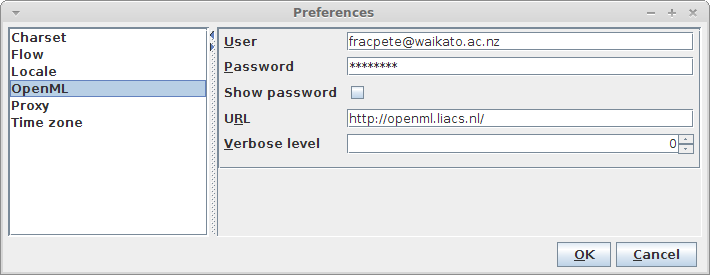
\includegraphics[width=8.0cm]{images/openml_preferences.png}
  \caption{OpenML preferences}
  \label{openml_preferences}
\end{figure}

%%%%%%%%%%%%%%%%%%%%%%%%%%%%%%%%%%%
% Copyright (c) 2009-2012 by the University of Waikato, Hamilton, NZ. 
% This work is made available under the terms of the 
% Creative Commons Attribution-ShareAlike 4.0 license,
% http://creativecommons.org/licenses/by-sa/4.0/.
%
% Version: $Revision$

\begin{thebibliography}{999}
	% to make the bibliography appear in the TOC
	\addcontentsline{toc}{chapter}{Bibliography}

    % references
	\bibitem{adams}
		\textit{ADAMS} -- Advanced Data mining and Machine learning System \\
		\url{https://adams.cms.waikato.ac.nz/}{}
		
	\bibitem{dl4j}
		\textit{deeplearning4j} -- open-source, distributed,
		deep-learning library for the JVM. \\
		\url{http://deeplearning4j.org/}{}

	\bibitem{json}
		\textit{JSON} -- JavaScript Object Notation is a lightweight data-interchange format \\
		\url{http://json.org/}{}

	\bibitem{yaml}
		\textit{YAML} -- is a human friendly data serialization
                standard for all programming languages. \\
		\url{http://yaml.org/}{}

\end{thebibliography}


\end{document}
